\documentclass[runningheads]{llncs}
\usepackage{graphicx}
\usepackage{float}
\usepackage{hyperref,xcolor}
%\usepackage{fullpage}
\bibliographystyle{splncs04}

\renewcommand\UrlFont{\color{blue}\rmfamily}

\title{LearNet}
\author{Sbârcea Ștefan-Vladimir}
\institute{ Faculty of Computer Science, Alexandru Ioan Cuza University of Iasi
\email{stefan.sbarcea@info.uaic.ro}}

\begin{document}

\maketitle

\begin{abstract}
LearNet is an application created to help students or anyone who wants to learn Computer Networks. The application is designed so that users have quick access to a lot of information in the field and can interact with other enthusiasts at the same time.
\end{abstract}


\section{Introduction}
\par In this report we will discuss in detail about LearNet application. This application is a client-server application where clients can interact with each other through chat or find useful information about computer networks. Every client needs an existing account to enter the application or they can create one if they have an invite code. Every chat, account and informational data is saved in an SQLite database. The information about computer networks that is presented in the application is taken from Alboaie Lenuta and Panu Andrei Computer Networks courses from Faculty of Computer Science \cite{computernetworks}.
\par The structure of this paper is as follows: Section 2 describes the technologies used in the creation of the application. Section 4 describes the architecture of the application. In Section 5 we present some implementation details including parts of the source code. Finally we draw some conclusions.

\section{Used technologies}
\par The application source code is written in C++ programming language.
\par To achieve the client-server connection we used the concurrent TCP model ( multi-processing), which allows the possibility of connecting several clients to the server and TCP’s reliable
data transfer service ensures that the data stream that a process reads out of its TCP receive buffer is uncorrupted, without gaps, without duplication, and in sequence; that is, the byte stream is exactly the same byte stream that was sent by the end system on the other side of the connection \cite{kurose1986computer}. 
\par The client GUI was made with Qt Creator, a cross-platform integrated development environment (IDE) built for the maximum developer experience \cite{qtcreator}. 
\par To save the information we used SQLite database because it is lightweight when it comes to setup complexity and resource usage \cite{kreibich2010using}. 
\section{Application architecture}
\par As we said prior the connection between server and client is done with TCP protocol and we create different processes to be able to serve clients concurrently. The server gets requests from the client it processes them and send back the data resulted. We created a database to save every client account information ( username, password, rank, chats and chat messages) and the information about computer networks. In figure 1 you can see how the connection between server-client was made and in figure 2 are presented the inside workings of the application. 

\begin{figure}[H]
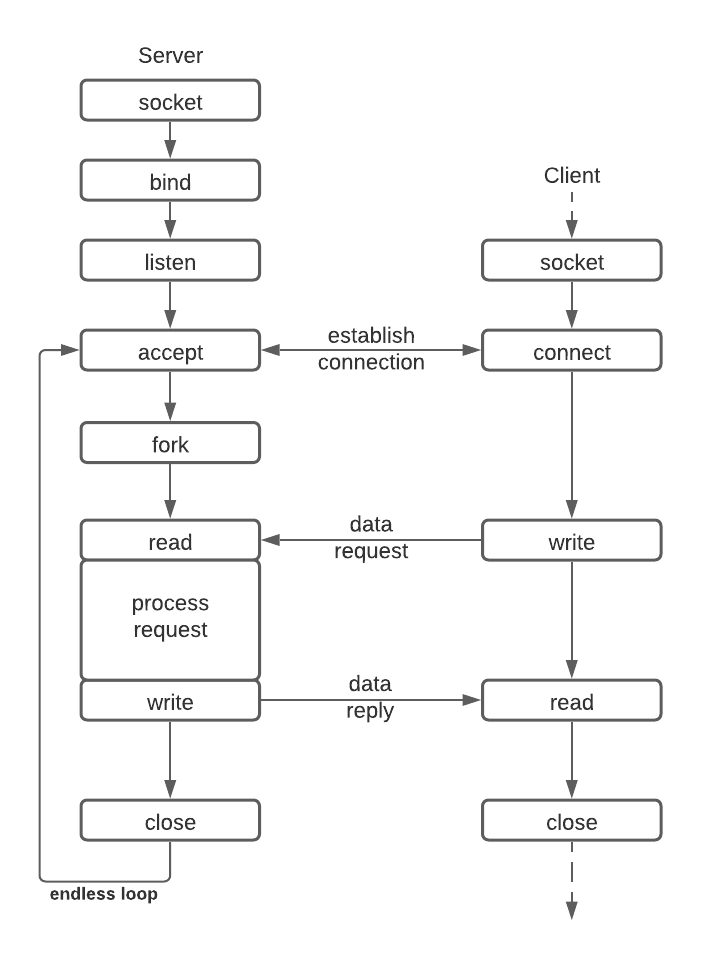
\includegraphics[width=\textwidth, height=5.2in]{images/client-server.png}
\caption{Application diagram}
\end{figure}
\begin{figure}[H]
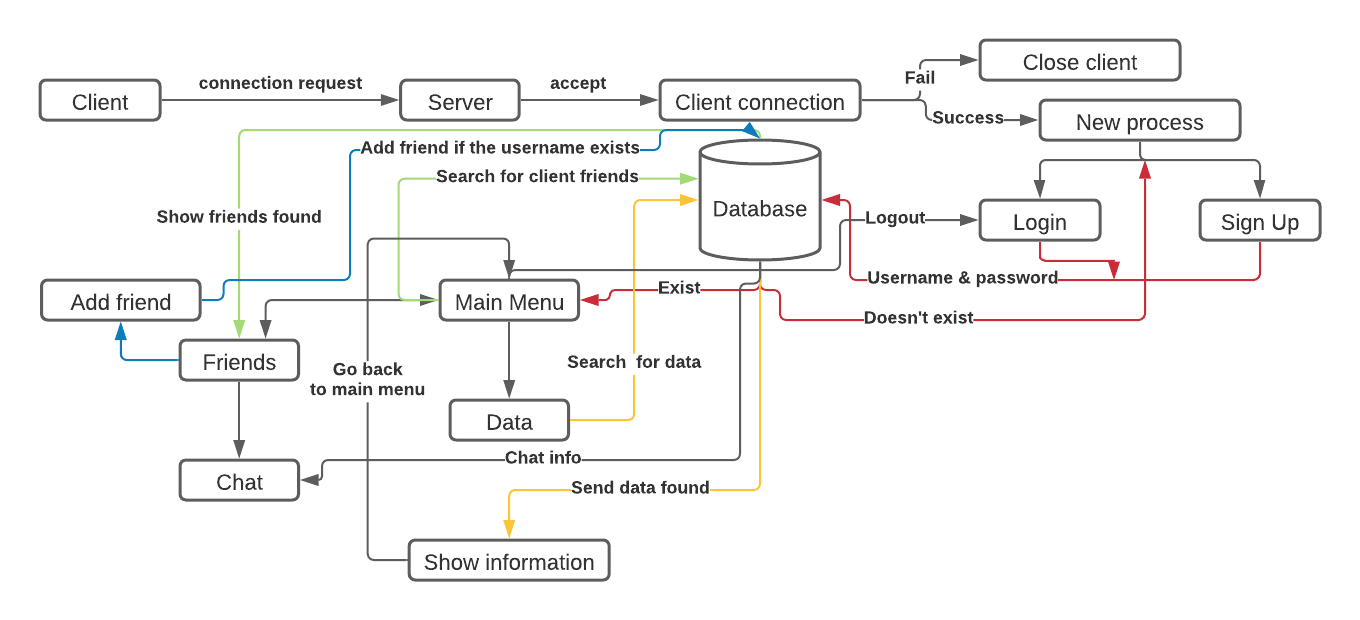
\includegraphics[width=6.6in, height=3.3in]{images/application.png}
\caption{Application diagram}
\end{figure}
\newpage
\par When the user starts the application it automatically connects to the server, if the server is not running it will throw an error, and the login/sign up menu will appear ( figure 3 )
\begin{figure}[H]
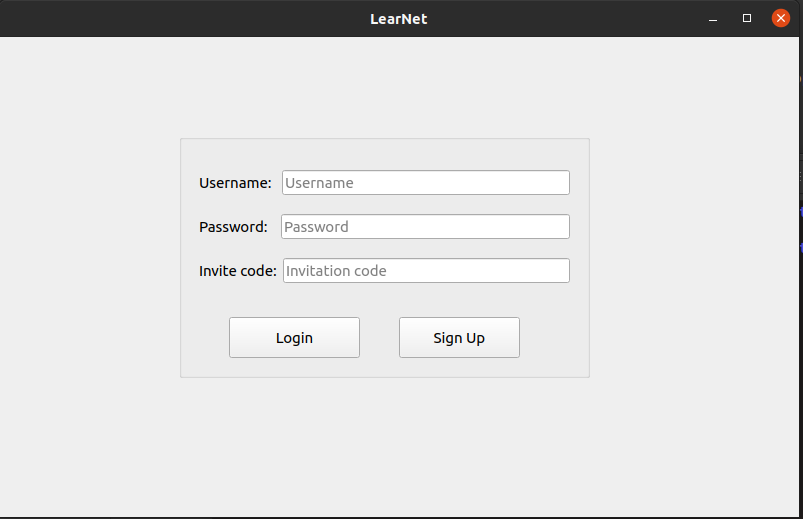
\includegraphics[width=\textwidth,height=\textheight,keepaspectratio]{images/login-signup.png}
\caption{Application login/sign up}
\end{figure}
, as said prior, if the user doesn't have an account he can create one by providing an username that doesn't exists in the database with a password and a valid invitecode, that can be obtained from a friend that has the permission to generate one, if the username already exists, the invite code is incorrect or the password doesn't respect the minimum requirements a specific warning will pop-up ( figures 4-5). After successfully signing up the user will be automatically logged in the application. ( figure 6)

\begin{figure}[H]
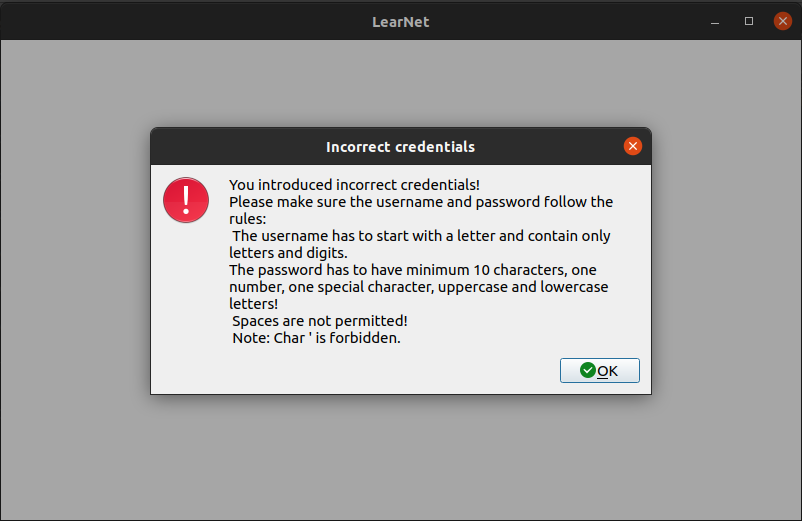
\includegraphics[width=\textwidth,height=\textheight,keepaspectratio]{images/incorrectCredentials.png}
\caption{Incorrect Credentials warning}
\end{figure}

\begin{figure}[H]
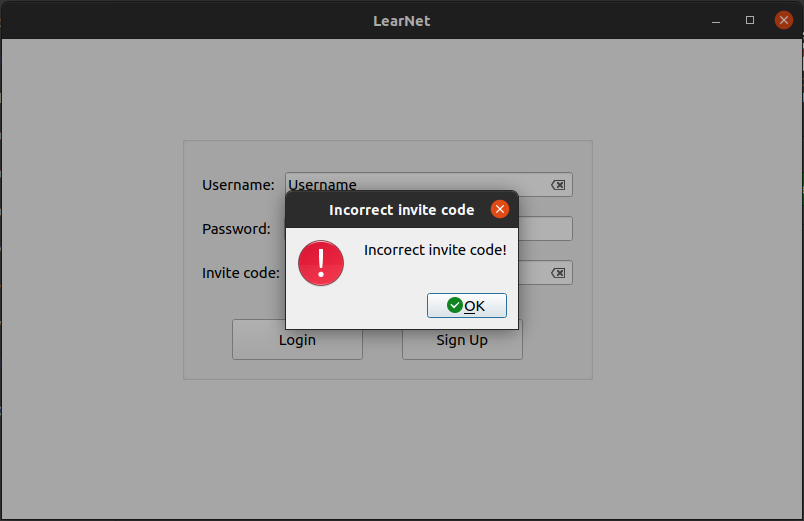
\includegraphics[width=\textwidth,height=\textheight,keepaspectratio]{images/incorrectInvitecode.png}
\caption{Incorrect Invite code warning}
\end{figure}

\begin{figure}[H]
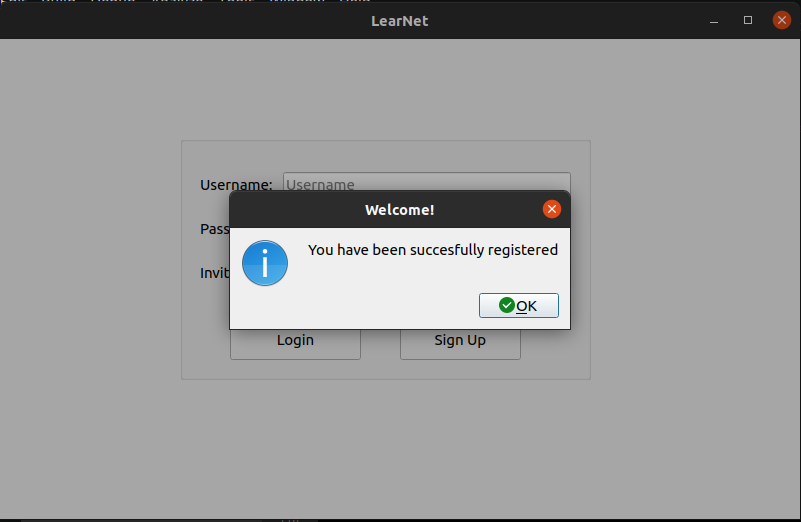
\includegraphics[width=\textwidth,height=\textheight,keepaspectratio]{images/succesfullyRegistered.png}
\caption{Successfully registered message box}
\end{figure}

The users that already have an account can just press on "Login" after completing the "Username:" and "Password:" fields ( the "Invite code:" field is ignored in this case), after pressing the "Login" button a pop-up will appear, if the username exists and the password is correct ( is the same with the one introduced at the creation of the account) a "Welcome!" message box will appear ( figure 7) and after closing it the user will be redirected to the application main menu, otherwise a warning will appear ( figure 8)
\newpage

\begin{figure}[H]
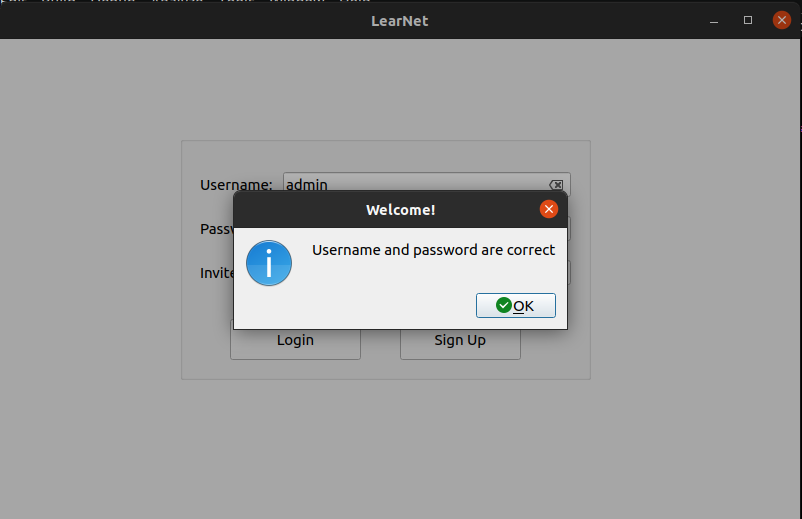
\includegraphics[width=\textwidth,height=\textheight,keepaspectratio]{images/correctUsernameOrPassword.png}
\caption{Welcome! message box}
\end{figure}


\begin{figure}[H]
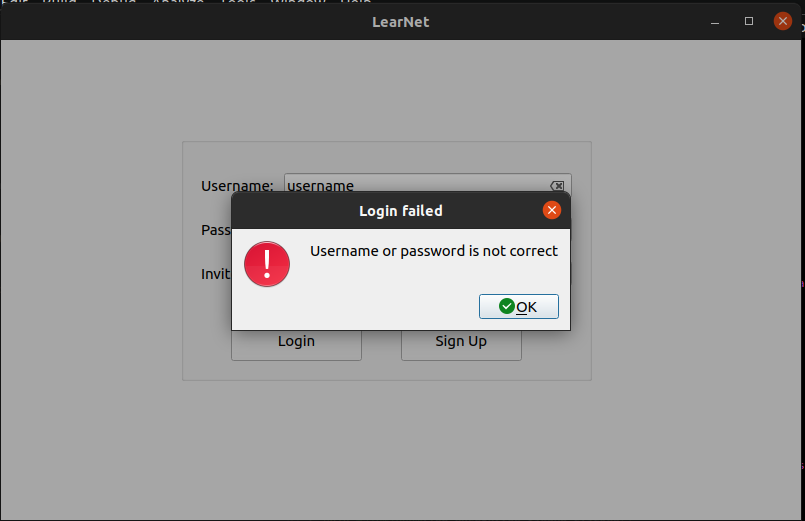
\includegraphics[width=\textwidth,height=\textheight,keepaspectratio]{images/incorrectUsernameOrPassword.png}
\caption{Login failed warning}
\end{figure}

The main menu ( figure 9) has 4 different buttons, the "Logout" button redirect the user to the login/sign up menu, the "Friends" button redirect the user to the friend list where it can add, remove or message a friend and generate an invite code if he has the permission ( figure 10), the "Search" button helps the user find the information he wants, of course if it exists in the database, and finally the "Open chat" button will open the all chat selected on the list located to the left of the "Open chat" button ( figure 11)

\begin{figure}[H]
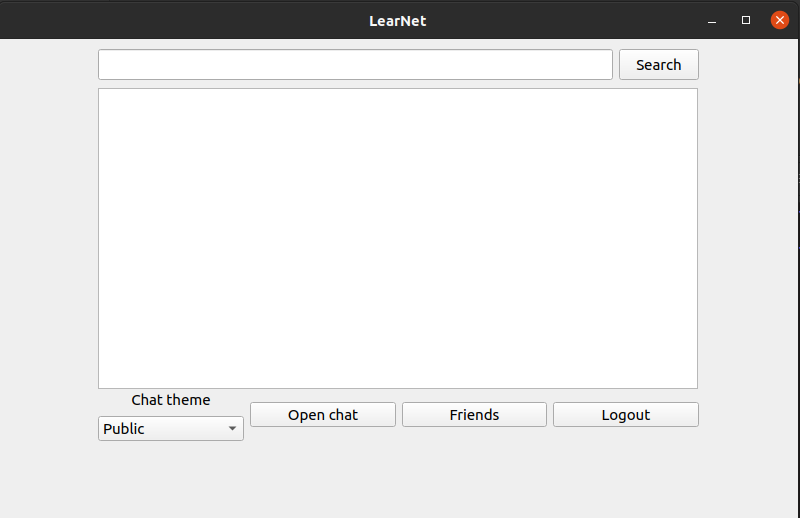
\includegraphics[width=\textwidth,height=\textheight,keepaspectratio]{images/mainmenu.png}
\caption{Main menu}
\end{figure}

\begin{figure}[H]
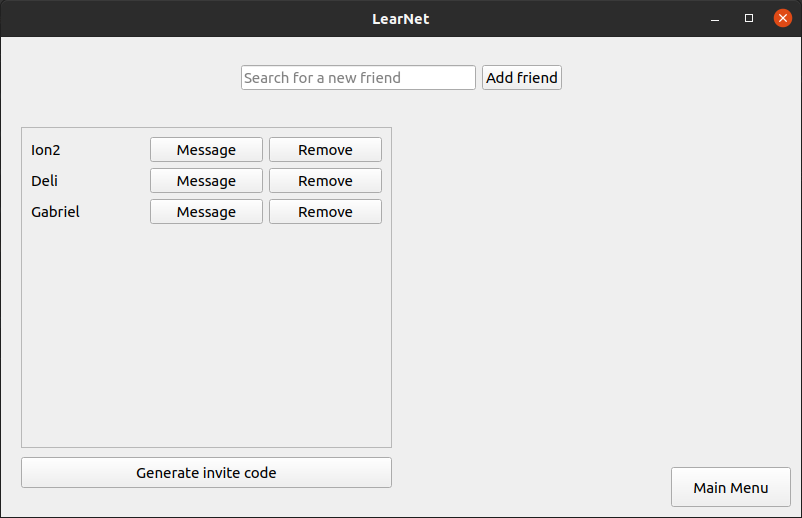
\includegraphics[width=\textwidth,height=\textheight,keepaspectratio]{images/friendsmenu.png}
\caption{Friends menu}
\end{figure}

\begin{figure}[H]
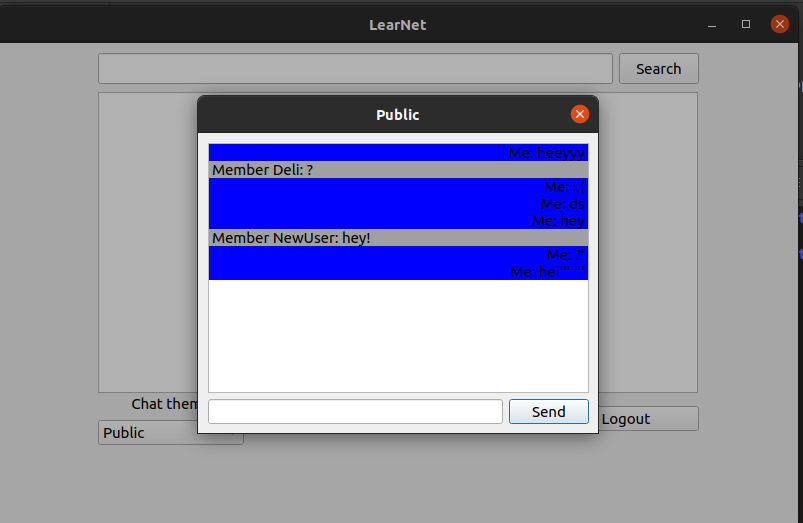
\includegraphics[width=\textwidth,height=\textheight,keepaspectratio]{images/allchat.png}
\caption{All chat}
\end{figure}

\par As you have seen in the application diagram ( figure 2) the database stands in the center of the implementation, in figure 12 we show how the database was designed. The chats between individual users are saved as different tables for every two users, that's why only the table \textbf{chats} appears in the diagram, which is used to save messages from every global chat. The \textbf{id} is unique and the \textbf{username} and
\textbf{type} are primary keys.

\begin{figure}[H]
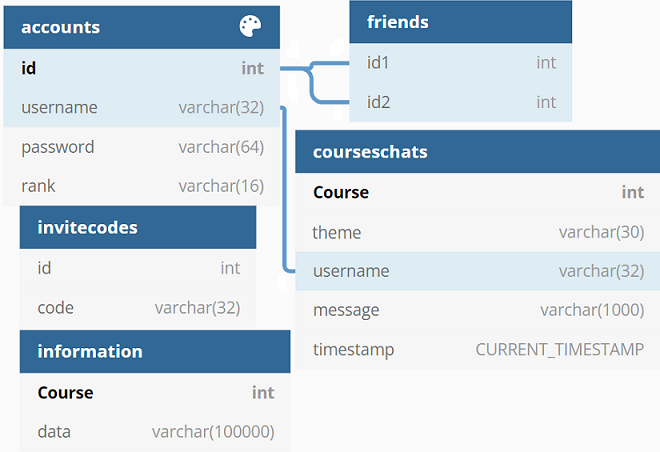
\includegraphics[width=\textwidth,height=\textheight,keepaspectratio]{images/dbdiagram.png}
\caption{Database diagram}
\end{figure}


\par The \textbf{invitecodes} table is used for sign up, only clients with an invite code are able to create a new account and every invite code is generated by an user with the specific rank.

\newpage
\section{Implementation details}

\subsection{Implementation use cases}

\begin{itemize}


\item \textbf{Use case 1:} Search for data\\
\textbf{Actor:} Student\\
\textbf{Basic Flow:} A student decides to use the application to search for a piece of information he couldn't find elsewhere. He starts the application, login into his account, searches for the information and finds it.\\
\textbf{Alternative Flow 1:} He notices that he doesn't have an account so he needs an invite code to create one.\\
\textbf{Alternative Flow 2:} He doesn't find the information, so he asks for that information in the chat.

\item \textbf{Use case 2:} Need help\\
\textbf{Actor:} Student\\
\textbf{Basic Flow:} A student needs help for a project related to computer networks, he asks on the LearNet application chat for help and someone helps him.\\
\textbf{Alternative Flow 1:} He doesn't want everyone to see what he doesn't know because it might make him look stupid so he adds the user to his friend list and speaks with him  in private.



\end{itemize}
\subsection{Implementation}
\par The server source code is split in 8 files:
\begin{enumerate}
\item \textbf{utilities.h} - used as an umbrella, containing every library needed and 5 utility functions: \textbf{handle\_ error(char*), int readBytes(int, char *, unsigned int), void recvMsg(int, char *), void sendMsg(int, char *), replaceAll}(std::string \& , const std::string \& , const std::string \& );
\item \textbf{utilities.cpp} - contains the implementation of the functions mentioned above;
\item \textbf{dbutilities.h} - contains the definition of the functions needed to save or take data from database;
\item \textbf{dbutilities.cpp} - contains the implementation of the functions from point 4;
\item \textbf{server.h} - contains the \textbf{Server} class;
\item \textbf{server.cpp} - contains the implementation of the \textbf{Server} class constructor and the following functions: \textbf{ void Server::acceptClients(), void Server::executeClient(int, char *), void Server::acceptClientsThreads()};
\item \textbf{commands.cpp} - contains the implementation of the \textbf{Server} class functions that analyze the data received from clients;;
\item \textbf{main.cpp} - contains the main function.
\end{enumerate}

\par The client source code is split in 13 files:

\begin{enumerate}

\item \textbf{client.h} - contains the \textbf{Client} class used for the connection between server and client;
\item \textbf{client.cpp} - contains the implementation of the \textbf{Client} class;
\item \textbf{mainwindow.h} - contains the \textbf{MainWindow} class;
\item \textbf{mainwindow.cpp} -  contains the implementation of the \textbf{MainWindow} class;
\item \textbf{mainwindow.ui} - stores the forms of the application login/sign up window in XML format;
\item \textbf{application.h} - contains the \textbf{Application} class;
\item \textbf{application.cpp} - contains the implementation of the \textbf{Application} class;
\item \textbf{application.ui} - stores the forms of the application main window in XML format;
\item \textbf{chat.h} - contains the \textbf{Chat} class
\item \textbf{chat.cpp} - contains the implementation of the \textbf{Chat} class;
\item \textbf{chat.ui} - stores the forms of the application chat window in XML format;
\item \textbf{interface.pro} - it's a multiplatform project file which qmake turns into platform-specific makefiles;
\item \textbf{main.cpp} - contains the main function.
\end{enumerate}

\par Every byte stream, sent between clients and server, is prefixed by his length as shown in figure 13, where \textbf{readBytes(int,char*,unsigned int)} function is used to read byte by byte the information so as not to lose data. 


\begin{figure}[H]
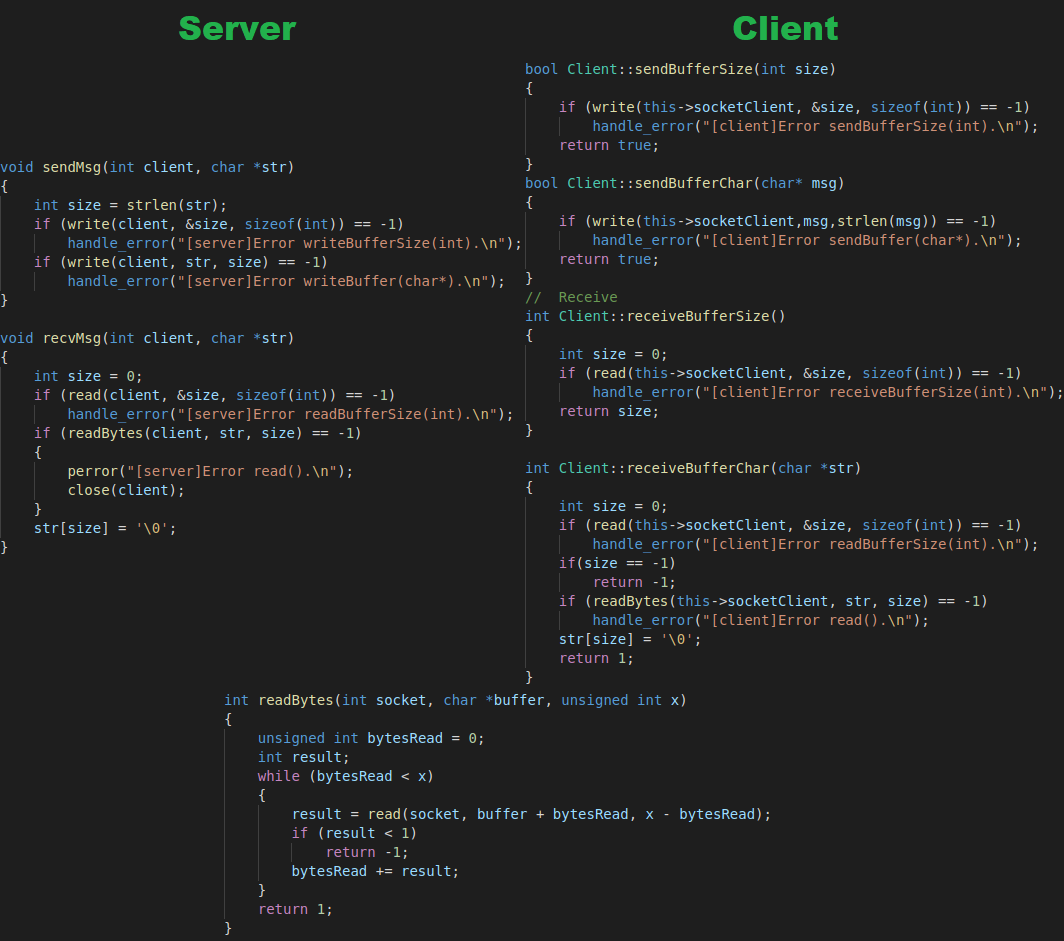
\includegraphics[width=\textwidth,height=\textheight,keepaspectratio]{images/sendRecv.png}
\caption{Send and receive functions server-client}
\end{figure}

\newpage 
\par We decided to explain and show how the login works. The client sends the command "login", the username and the password to the server and waits for the server to respond ( figure 14). The server checks the command and calls function \textbf{login(int)} where it reads the username and password and searches for them in the database to see if there is a match in \textbf{accounts} table the function \textbf{searchUsrAndPwd(database, username, password)} returns -1 on failure and the user id on success ( 0$\leq$id) ( figure 15).

\begin{figure}[H]
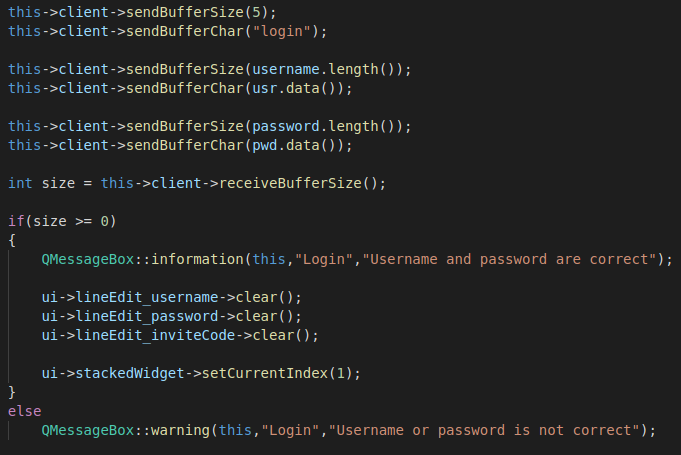
\includegraphics[]{images/client-login.png}
\caption{Client-login}
\end{figure}

\newpage 
\begin{figure}[H]
\begin{center}
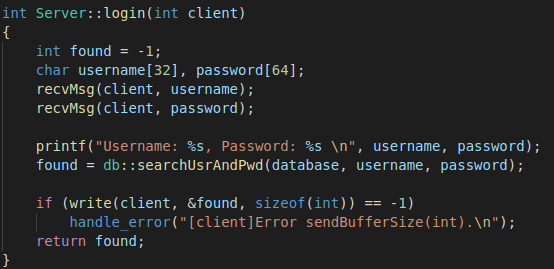
\includegraphics[]{images/server-login.png}
\caption{Server-login}
\end{center}
\end{figure}

\par Another important part of the source code is the generation of the chats between users that is shown in the following figures ( figure 6 and 7). The client creates a new object \textbf{Chat} and fills it with the messages the server provides from the database, if there are any. 

\begin{figure}[H]
\begin{center}
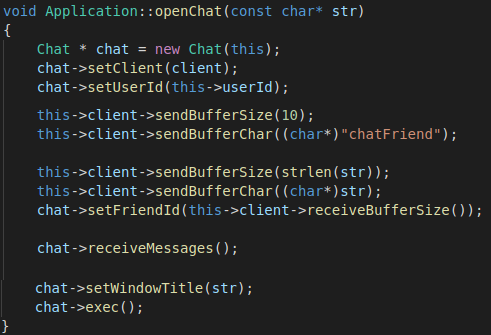
\includegraphics[]{images/client-chat.png}
\caption{Client-chat}
\end{center}
\end{figure}

\newpage

\begin{figure}[H]
\begin{center}
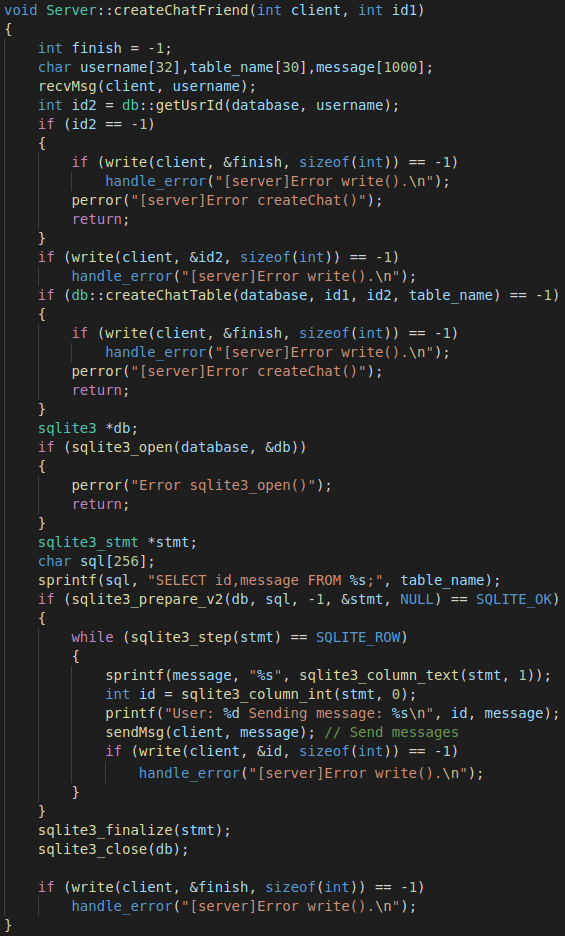
\includegraphics[]{images/server-chat.png}
\caption{Server-chat}
\end{center}
\end{figure}

\section{Conclusions}

This application can be very useful for people passionate about computer networks, because it offers a decent amount of information about the subject and it gives you the option to discuss about the subject with other people interested in this topic. An upgrade that can be done to this application would be the possibility to up vote useful messages or user profiles to show how involved they are in the community or how trusted they can be when asking for an advice or help in global chats. 

\bibliography{ref.bib}

\end{document}